\chapter{Softwareprozesse}
Softwareprozess ist eine Menge von zusammengehörigen Aktivitäten, die zur Produktion eines Softwareprodukts führen.
\section{Vier Aktivitäten die grundlegend für SE sind:}
\begin{itemize}
    \item Softwarespezifikation:
    \begin{itemize}
        \item Beschreibung was das System macht
    \end{itemize}
    \item Softwareentwurf und -implementierung
    \begin{itemize}
        \item Definieren des Systemaufbaus
        \item Implementierung des Systems
    \end{itemize}
    \item Softwarevalidierung
    \begin{itemize}
        \item Sind Kundenwünsche erfüllt
    \end{itemize}
    \item Softwareevolution
    \begin{itemize}
        \item Weiterentwicklung und eingehen auf veränderte Bedürfnisse des Kunden
    \end{itemize}
\end{itemize}

\section{Plangesteurte und agile Prozesse:}
\begin{itemize}
    \item Plangesteurte Prozesse:
    \begin{itemize}
        \item Verfahren bei denen alle Prozessaktivitäten im Voraus geplant werden
        \item Fortschritte werden an dem Plan gemessen
    \end{itemize}
    \item Pro:
    \begin{itemize}
        \item durch frühzeitige Planung werden Probleme und Abhängigkeiten entdeckt\\
         (z.B. Personalbedarf)
    \end{itemize}
    \item Contra:
    \begin{itemize}
        \item viele frühe Entscheidungen müssen korrigiert werden \\
        (z.B. wegen Änderungen in der Umgebung)
    \end{itemize}
    \item Agile Prozesse:
    \begin{itemize}
        \item Planen ist inkrementell und es ist einfacher Prozesse zu verändern 
    \end{itemize}
    \item Es muss eine Balance zwischen beiden Prozessen gefunden werden
\end{itemize}

\section{Vorgehensmodelle (Softwareprozessmodelle):}
\begin{itemize}
    \item Wasserfallmodell
    \item Inkrementelle Entwicklung 
    \item Wiederverwendungsorientierte SE
\end{itemize}

\subsection{Wasserfallmodell:}
\begin{figure}[h] 
  \centering
     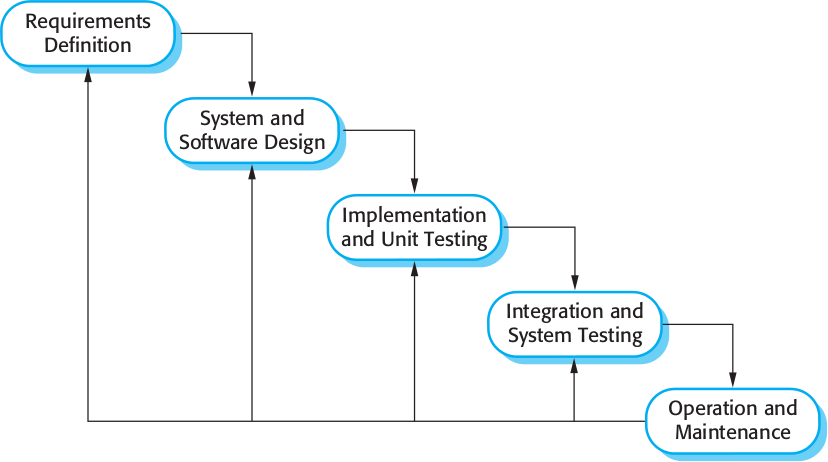
\includegraphics[width=0.75\textwidth]{mainmatter/pics/waterfall.png}
  \caption{Wasserfallmodell: Plangesteuerter Prozess}
\end{figure}
\begin{itemize}
    \item Modell stellt die grundlegende Prozessabläufe (Spezifikation, Entwicklung, Validierung und Evolution) als eigene Phase des Prozesses dar
    \item Phasen
    \begin{enumerate}
        \item Analyse und Definition der Anforderungen dienen als Systemspezifikation
        \item System- und Softwareentwurf:
        \begin{itemize}
            \item Übergeordnete Systemarchitektur wird festgelegt
            \item Erkennen und Beschreiben  der grundlegenden abstrakten Softwaresysteme 
        \end{itemize}
        \item Implementierung und Modultests
        \item Integration und Systemtest
        \begin{itemize}
            \item System wird als Ganzes getestet zur Siherheitsstellung, dass die Softwareanforderungen erfüllt sind. 
        \end{itemize}
        \item Betrieb und Wartung
    \end{enumerate}
    \item Hauptproblem ist die starre Aufteilung des Projekts in verschiedene Phasen
    \item Man kann nicht gut auf neue Anforderungen des Kunden reagieren
    \item gute \glqq{}Wahl\grqq{}, wenn Anforderungen gut durchdacht sind und wenn keine Änderungen zu erwarten sind
    \item geeignet für große Systeme
\end{itemize}

\subsection{Inkrementelle Entwicklung}
\begin{itemize}
    \item Spezifikation, Entwicklung und Validierung sind verschachtelt. Kann sowohl plangesteuertals auch agil sein.
    \item System wird als eine Folge von Versionen (Inkrementen) entwickelt, wobei jede Version neue Funktionalität zu der vorherigen hinzufügt
    \item Spezifikation, Entwicklung und Validierung werden gleichzeitig ausgeführt
\end{itemize}
\begin{figure}[h] 
  \centering
     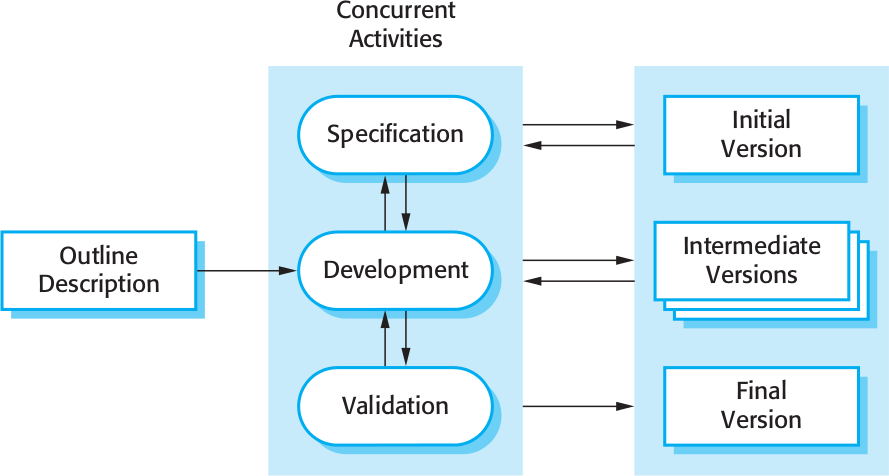
\includegraphics[width=0.75\textwidth]{mainmatter/pics/inkrement_evolution.png}
  \caption{Inkrementelle Entwicklung}
\end{figure}
\textbf{Vorteile inkrementelle Entwicklung (gegenüber Wasserfallmodell):}
\begin{itemize}
    \item Kosten für Kundenanforderungsänderungen werden reduziert
    \item Es ist einfacher Kundenrückmeldungen zu bekommen 
    \item Schnellere Auslieferung an den Kunden von verwendungsfähiger Software 
\end{itemize}

\textbf{Nachteile inkrementelle Entwicklung}
\begin{itemize}
    \item Prozess ist nicht sichtbar
    \begin{itemize}
        \item Fortschritt nicht messbar
    \end{itemize}
    \item Systemstruktur wird tendenziell schwächer, wenn neue Inkremente hinzugefügt werden
\end{itemize}
\subsection{Inkrementelle Lieferung}
\begin{itemize}
    \item Entwicklung und Auslieferung werden in mehrere Schritte aufgeteilt, jeder Schritt liefert einen Teil der geforderten Funktionalitäten
    \item Den Benutzeranforderungen werden Prioritäten zugewiesen, die Anforderungen mit höherer Priorität werden in früheren Schritten bearbeitet 
    \item während der Bearbeitung eines Schrittes werden die betreffenden Anforderungen nicht mehr verändert
\end{itemize}
\begin{figure}[h] 
  \centering
     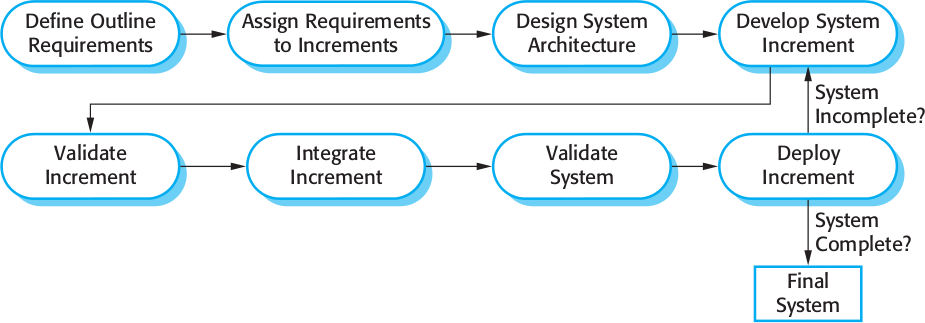
\includegraphics[width=0.75\textwidth]{mainmatter/pics/inkrement_delivery.png}
  \caption{Inkrementelle Lieferung}
\end{figure}
\textbf{Vorteile:}
\begin{itemize}
    \item Schrittweise gelieferte Systemfunktionalität
    \item Frühe Schritte dienen als Vorlage, mit der spätere Schritte bestimmt werden
    \item Geringes Risiko für Fehlschlag der gesamten Software 
    \item die hoch priorisierten Systemdienstleistungen werden oft getestet
\end{itemize}
\textbf{Nachteile:}
\begin{itemize}
    \item Schwer zu verwalten
\item  Systemstruktur wird aufgeweicht
\item  Kompatibilität mit Geschäftsprozessen auf Kundenseite nicht gesichert
\item  Ersetzen eines bestehenden Systems problematisch $\rightarrow$ Schritte enthalten weniger Funktionalität
\end{itemize}

\subsection{Wiederverwendungsorientiertes Software Engineering}
\begin{figure}[h] 
  \centering
     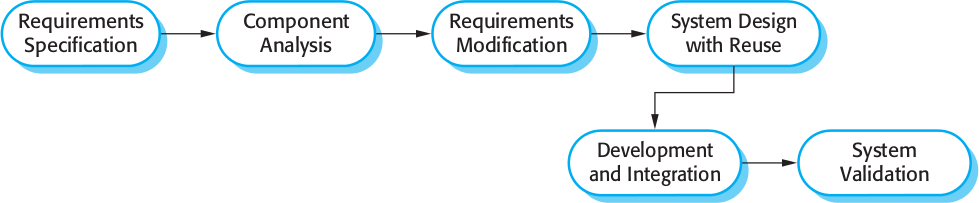
\includegraphics[width=0.75\textwidth]{mainmatter/pics/reused.png}
  \caption{Reuseoriented software engineering}
\end{figure}


\begin{itemize}
    \item beides (Plandriven \& agiler Prozess)
    \item basiert auf Existenz einer beträchtlichen anzahl von wiederverwendbaren Komponenten 
    \item Prozessstufen: 
    \begin{itemize}
        \item Komponenten Analyse
        \item Anforderungsmodifikation
        \item Systementwurf mit Wiederverwendung 
        \item Entwicklung und Integration
    \end{itemize}
    \item meist aus allen Modellen zusammengesetzt
\end{itemize}

\subsection{Typen der Software-Komponenten:}
\begin{itemize}
    \item Stand-Alone-Software (COTS Commercial-off-the-shelf):\\
    wurde für den Einsatz in einer bestimmten Umgebung Entwickelt
    \item Sammlung von Objekten, die als Paket mit einem Komponentenframework wie .NET oder J2EE integriert und entwickelt wurden
    \item Web-Services:\\
    wurden je nach Servicestandard entwickelt und für Remote-Aufrufe verfügbar gemacht
\end{itemize}

\section{Prozessaktivitäten:}
\subsection{Softwarespezifikation}
Prozess zum Verstehen und Definieren der vom System verlangten Funktion sowie der Beschränkungen, denen der Betrieb und die Entwicklung des Systems unterliegen. 
\\
\textbf{Requirements Engineering}
\begin{enumerate}
    \item Anforderungsanalyse besteht aus 
    \item \textbf{Durchführbarkeitsstudie:}
    \begin{itemize}
        \item Ist es aus technischer und finanzierler Sicht möglich das System zu entwickeln?
    \end{itemize}
    \item \textbf{Erhebung und Analyse der Anforderungen:}
    \begin{itemize}
        \item Was erwarten die Kunden von dem System 
    \end{itemize}
    \item \textbf{Spezifikation der Anforderungen:}
    \begin{itemize}
        \item Definieren der Anforderungen im Detail
    \end{itemize}
    \item \textbf{Validierung der Anforderungen:}
    \begin{itemize}
        \item Sind die Anforderungen realistisch, konsistent und vollständig?
    \end{itemize}
\end{enumerate}
\begin{figure}[h] 
  \centering
     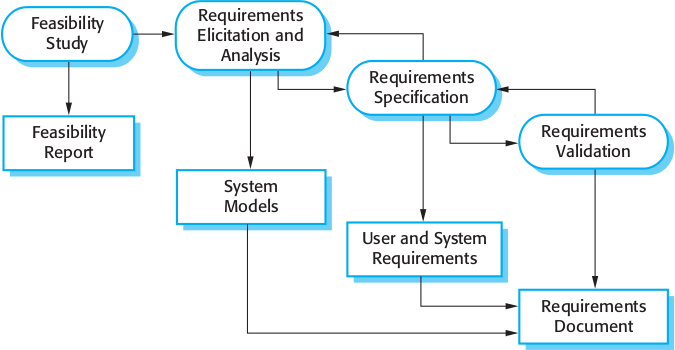
\includegraphics[width=0.75\textwidth]{mainmatter/pics/requ.png}
  \caption{Softwarespezifikationen}
\end{figure}

\subsection{Design und Implementierung}
Umwandlen der Spezifikationen in ein ausführbares System.
\begin{itemize}
\item Software-Design
    \begin{itemize}
        \item  Entwicklung einer Softwarestruktur, die die Spezifikation umsetzt.
    \end{itemize}
\item Implementierung
    \begin{itemize}
        \item Übersetzung der Struktur in ein ausführbares Programm.
    \end{itemize}
\end{itemize}
\begin{figure}[h] 
  \centering
     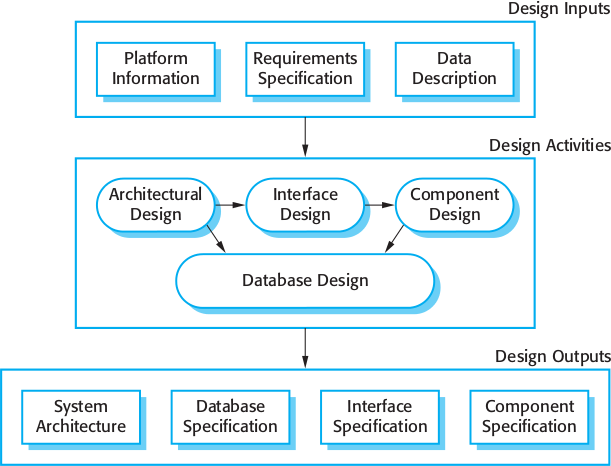
\includegraphics[width=0.75\textwidth]{mainmatter/pics/entw_impl.png}
  \caption{Design und Implementierung}
\end{figure}

\subsection{Designaktivitäten
}
\begin{itemize}
    \item Architekturentwurf:\\
    Gesamtstruktur des Systems $\rightarrow$ Hauptkomponenten (wie Untersysteme und Module), Beziehungen und deren Verteilungen
    \item Schnittstellenentwurf:\\
    Definition der Schnittstellen zwischen Systemkomponenten
    \item Komponentenentwurf:\\
    Jede Komponente und jedes Design wird genauer betrachtet
    \item Datenbankentwurf:\\
    Entwurf der Systemdatenstruktur und deren Darstellung in der Datenbank
\end{itemize}
\subsection{Software- Validierung}
\begin{itemize}
    \item Verfikation und Validierung soll zeigen, dass ein Systeseiner Spezifikation entspricht und die Anfoerderungen des Kunden erfüllt
    \item Kontrolle und Bewertungsprozess, Testendes Systems 
    \item Testing: ausführen des Systems mit Testfällen (aus der Spezifikation der Daten, die mit dem System verarbeitet werden sollen)
    \item \textcolor{red}{Häufigste V\&V-Aktivität: Testing}
\end{itemize}
\begin{figure}[h]
  \centering
     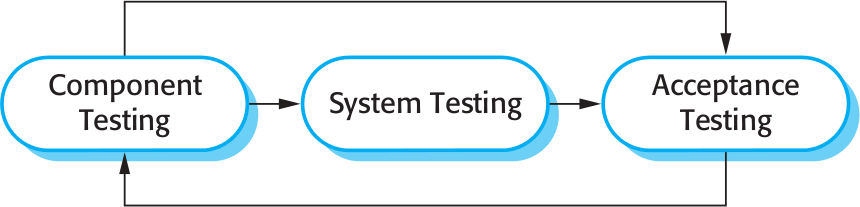
\includegraphics[width=0.75\textwidth]{mainmatter/pics/vandv.png}
  \caption{Testing Zyklus}
\end{figure}
\begin{itemize}
    \item Komponenten Testing:
    \begin{itemize}
        \item Tests von Einzelkomponenten unabhängig von einander
        \item Komponenten können Funktionen, Objekte oder kohärente Gruppen von Personen sein
    \end{itemize}
    \item Systemtest
    \begin{itemize}
        \item Test des gesamten Systems (entstehender Eigenschaften)
        \item Prüfung von emergenten Eigenschaften besonders wichtig
    \end{itemize}
    \item Abnahmetests:
    \begin{itemize}
        \item Testen mit Daten des Kunden zur Überprüfung der Anforderungen
    \end{itemize}
\end{itemize}
\begin{figure}[h]
  \centering
     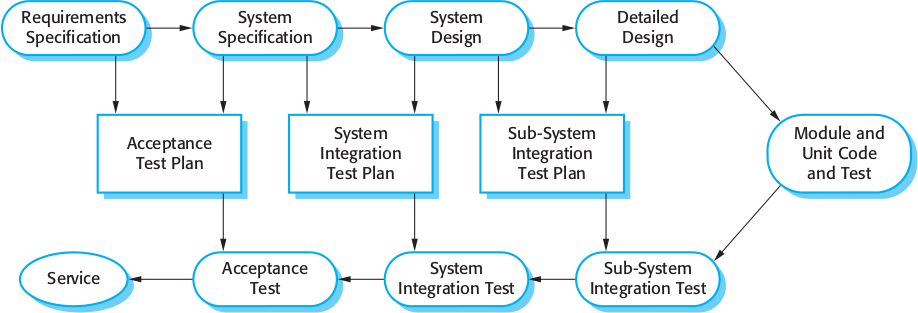
\includegraphics[width=0.75\textwidth]{mainmatter/pics/validation.png}
  \caption{Testing bei plangesteuertem Software-Prozess}
\end{figure}

\subsection{Key Points:}
\begin{enumerate}
    \item Softwareprozesse sind Aktivitäten, die zur Entwicklung neuer Software gehören. Software-Prozessmodelle sind die abstrakten Repräsentationen dieser Prozesse. 
    \item Prozessmodelle beschreiben die Organisation von Softwareprozessen. (Wasserfall, inkrementelle Entwicklung, Wiederverwertungs-orientierte Entwicklung) 
    \item Requirements Engineering: Entwicklung einer Software-Spezifikation 
    \item Design und Implementierung wandeln die Anforderungs-Spezifikation in ein ausführebares Softwaresystem um. 
    \item Validierung: Erfüllung der Sytem-Spezifikation und der Kundenwünsche wird überprüft
    \item Evolution: Veränderung existierender Systeme zur Erfüllung 
\end{enumerate}


\subsection{Software-Evolution}
\begin{itemize}
    \item Software ist von Natur aus flexibel und kann sich verändern
    \item Anforderungen änder sich durch wirtschafliche Umstände, die unterstützende Software muss sich mit verändern
    \item Durch die Wiederverwendung von Komponenten für neue Systeme sind Softwareentwicklung und Evolution nicht mehr vollständig unterscheidbar
\end{itemize}
\begin{figure}[h]
    \centering
    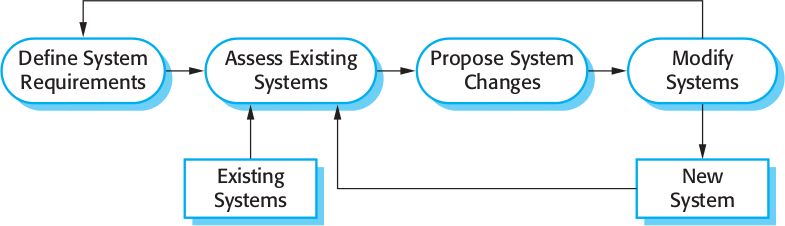
\includegraphics[width=0.75\textwidth]{mainmatter/pics/evolution.png}
    \caption{Software-Evolution}
\end{figure}


\section{Bewältigung von Veränderungen}
Veränderungen führen zu Nacharbeit. Die Veränderungskosten beinhalten Nacharbeit und Implementierung neuer Funktionalitäten
\subsection{Kostenreduzierung}
\begin{itemize}
    \item \textbf{Change avoidance:} vorwegnehmen möglicher Veränderungen
    \item \textbf{Change tolerance:} Gesamtprozess kann Veränderungen leicht umsetzen
\end{itemize}
\subsection{Prototyping}
\begin{figure}[h]
    \centering
    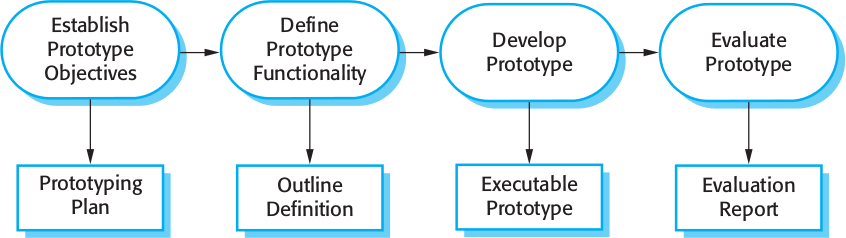
\includegraphics[width=0.75\textwidth]{mainmatter/pics/prototyping.png}
    \caption{Prototyping}
\end{figure}
\begin{itemize}
    \item Demonstration von Konzepten und ausprobieren von Designmöglichkeiten
    \item Wird benutzt, wenn:
    \begin{itemize}
        \item Requirements-Engineering Prozess hilft ein Prototyp bei der Ermittlung und Validierung der Systemanforderungen
        \item Beim Systementwurf kann der Prototyp verwendet werden, um einzelne Softwarelösungen zu untersuchen und den Entwurf der Benutzeroberfläche zu unterstützen 
    \end{itemize}
\end{itemize}

\qquad\\
\qquad\\
\subsection{Spiralmodell nach Boehm:}
\begin{figure}[h]
    \centering
    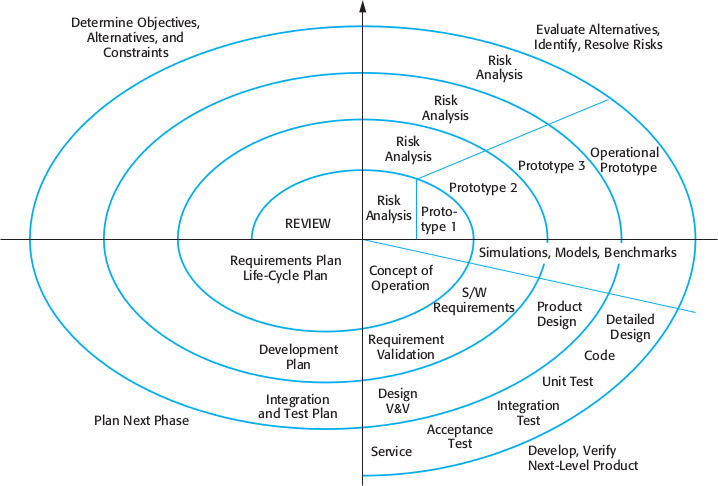
\includegraphics[width=0.75\textwidth]{mainmatter/pics/boehm.png}
    \caption{Spiralmodell nach Boehm}
\end{figure}

\begin{itemize}
    \item Softwareprozess wird als Spirale dargestellt, anstatt als eine Folge von Aktivitäten 
    \item Jede Windung steht für eine Phase des Prozesses
    \item keine festen Phasen wie Spzeifikation $\rightarrow$ Schleifen werden nach Erforderlichkeit gewählt.
    \item beinhaltet explizite Risikomanagmentaktivitäten
    \item Jede Windung der Spirale ist in vier Segmente aufgeteilt:
    \begin{itemize}
        \item Ziele aufstellen
        \item Risiken einschätzen und verringern
        \item Entwicklungnd Validierung
        \item Planung
    \end{itemize}
    \item \textbf{Risiken} werden während dem Prozess angesprochen und geklärt
    \item Nutzung:
    \begin{itemize}
        \item sehr einflussreich um Menschen zu helfen über Iterationen in Softwareprozessen und die Eifnührung des risikoorientierten Ansatzes für die Entwicklung nach zu denken
        \item Praxis
        \begin{arrowlist}
            \item Modell wird selten verwendet
            \item wird zur Veröffentlichung der praktischen Softwareentwicklung verwendet
        \end{arrowlist}
    \end{itemize} 
\end{itemize}





\subsection{Rational Unified Process (RUP):}
\begin{itemize}
    \item Generisches Verfahren
    \item abgeleitet von der Arbeit an der UML
    \item Vereinigt Elemente aus allen allgemeinen/generischen \textbf{Vorgehensmodellen} (Wasserfall, inkrementelle Entwicklung und wiederverwendungsorienteirte SE)
    \item veranschaulicht empfohlene Vorgehensweisen für Spezifikation und Entwurf
    \item unterstützt Entwicklung von Prototypen
    \item RUP wird aus drei Perspektiven beschrieben
    \begin{itemize}
        \item \textbf{dynamische Perspektive:}\\
        zeigt Entwicklungsphasen über die Zeit
        \item \textbf{statische Perspektive:}\\
        die die ausgeführten Prozessaktivitäten darstellt
        \item \textbf{praxisbezogene Perspektive:}\\ die die während des Prozesses empfohlene Vorgehensweise vorschlägt
    \end{itemize}
    \item Sechs grundlegende Vorgehensweisen für das SE zum Einsatz bei der Systementwicklung:
    \begin{enumerate}
        \item Software iterativ entwickeln:
        \begin{itemize}
            \item schrittweise Planung des Systems ausgehend von den Prioritäten des Kunden 
        \end{itemize}
        \item Anforderungen verwalten:
        \begin{itemize}
            \item Eindeutige Dokumentation der Kundenanforderungen
            \item geänderte Anforderungen verfolgen
        \end{itemize}
        \item Komponentenbasierte Architekturen verwenden:
        \begin{itemize}
            \item Aufteilung der Systemarchitektur in Komponenten (Wiederverwendung)
        \end{itemize}
        \item Software visuell modellieren:
        \begin{itemize}
            \item Verwenden grafischer UML-Modelle für dynamische und statische Sicht 
        \end{itemize}
        \item Softwarequalität verifizieren:
        \begin{itemize}
            \item Sicherstellen, dass die Software die Qulaitätsstandards des Unternehmens erfüllen
        \end{itemize}
        \item Änderungen der Software steuern (überprüfen):
        \begin{itemize}
            \item Verwaltung der Softwareveränderungen mithilfe eines Änderungsmanagementsystems
        \end{itemize}
    \end{enumerate}
\end{itemize}

\subsection{Key Points}
\begin{itemize}
\item Prozesse sollten Verfahren für den Umgang mit Veränderungen einbeziehen
\item Iterative Entwicklung und Auslieferung: Veränderungen können umgesetzt werden, ohne das Gesamtsystem zu beeinträchtigen
    \item Boehms Spiralmodell nimmt Rücksicht auf Risiken und Neuplanungen/Überarbeitungen
    \item RUP ist ein modernes allgemines Vorgehensmodell, das zwar in Phasen unterteil ist \textbf{(Konzeption, Entwurf, Konstruktion und ÜBergabe)}, jedoch die Aktivitäten (Anforderungsanalyse, Analyse und Entwurf) von den Phasen trennt
\end{itemize}
